%----------------------------------------------------------------------------------------
%    PACKAGES AND THEMES
%----------------------------------------------------------------------------------------

\documentclass[aspectratio=169,xcolor=dvipsnames]{beamer}
\usetheme{SimpleDarkBlue}

\usepackage{hyperref}
\usepackage{graphicx} 
\usepackage[labelformat=empty]{caption}

\usepackage{hw_beamer}% Allows including images
\usepackage{mypreamble}
\usepackage{booktabs} 
% \usepackage{hw}
% \usepackage{hw}
% \usepackage{amsmath}
% \usepackage{mathtools} % For \diag and other math operators
\newcommand{\Var}{\text{\textbf{Var}}}
\newcommand{\R}{\mathbb R}
\newcommand{\E}{\mathbb E}
\newcommand{\simiid}{\overset{iid}\sim }

%----------------------------------------------------------------------------------------
%    TITLE PAGE
%----------------------------------------------------------------------------------------

\title{Equispaced Fourier Features for Gaussian Processes}
% \subtitle{Scalable computation and inference in low dimensions}

\author{Cole Citrenbaum}

\institute
{
    % Department of Computer Science and Information Engineering \\
    % National Taiwan University % Your institution for the title page
}
\date{\today} % Date, can be changed to a custom date

%----------------------------------------------------------------------------------------
%    PRESENTATION SLIDES
%----------------------------------------------------------------------------------------
\usepackage{natbib}           % optional but common in Beamer


\bibliographystyle{plainnat}  % or abbrvnat, ieeetr, etc.
\begin{document}

\begin{frame}
    % Print the title page as the first slide
    \titlepage
\end{frame}

\begin{frame}{Overview}
    % Throughout your presentation, if you choose to use \section{} and \subsection{} commands, these will automatically be printed on this slide as an overview of your presentation
    \tableofcontents
\end{frame}


\section{Motivation}
\begin{frame}{Motivating example}
    \begin{figure}
        \centering
        \includegraphics[width=0.48\linewidth]{raw_mouse.png}
        \caption{Excitatory gene expression levels in mouse hippocampus}
    \end{figure}
\end{frame}

\begin{frame}{Weather Example}
    \begin{figure}
        \centering
        
\includegraphics[width=0.7\linewidth]{temperature_squared_exponential.png}
    \end{figure}
\end{frame}

\begin{frame}{Motivation}
Consider a Gaussian Process regression setup:

$$y|f = f(x) + \mathcal N(0,\sigma^2) \quad \text{ or } \quad y|f \sim \operatorname{Bern}(\sigma(f(x)) \quad \text{ etc},$$
$$f(X) \sim GP(0,K).$$

This setup is common in:
\begin{enumerate}
    \item Spatial statistics, meteorology
    \item Astrophysics
    \item Neuroscience (eg time series of firing rates)
    \item Spatial transcriptomics
\end{enumerate}
Benefits
\end{frame}




\begin{frame}{Challenges in GP regression}
Posterior mean and variance

$$\E[f(x_*)|y] = K(x_*,x)^T  (\textbf{K}+\sigma^2I)^{-1} y$$

$$  \Var [f(x_*)|y] = \textbf{K}(x_*, x_*) - \textbf{K}(x_*,\textbf{x})(\textbf{K}+\sigma^2 \textbf{I})^{-1}k(\textbf{x},x_*)$$

And gradients of log marginal:

$$\frac{d\cal L}{d\theta} = \frac{1}{2} \left( \tr \left( (K+\sigma^2 I)^{-1} \partial_\theta (K+\sigma^2 I)\right) - y^T (K+\sigma^2 I)^{-1} \partial_\theta (K+\sigma^2 I) (K+\sigma^2I)^{-1} y\right) $$

    Limited by $\mathcal O(n^3)$ cost of inverting $(K+\sigma^2 I)$ (eg Cholesky), rendering GP regression impractical in otherwise attractive scenarios. 
\end{frame}
\begin{frame}{Tools}
    
\end{frame}
\begin{frame}{Conjugate Gradients}
    Rather than computing $(K+\sigma^2 I)^{-1}y = \alpha $, we can compute via conjugate gradients. Solve:
    $$(K+\sigma^2 I)\alpha = y$$
    by iteratively applying $K+\sigma^2 I$ until convergence. \\ \vspace{0.5cm}
    Complexity $\mathcal O(n^2 m)$
\end{frame}

\section{Background - Equispaced Fourier Features}
\begin{frame}{Kernel Fourier Approximations}

Bochner's Theorem guarantees existence of a spectral density $\hat k$ for stationary kernels:

$$k(x ,x') = \int \hat{k}(\xi) \exp(2\pi i \xi(x-x') ) d\xi, \quad \tau \in \R^d$$

A natural idea is to approximate:
\begin{align}k(x,x') \approx \sum_{\ell=1}^m w_\ell \hat{k}(\xi_\ell) \exp(2\pi i \xi_\ell (x - x') )&= \sum_{\ell=1}^m \sqrt{w_\ell \hat k (\xi_\ell)}\exp(2\pi i\xi_\ell x)\sqrt{w_\ell \hat k (\xi_\ell)}\exp(-2\pi i \xi_\ell x') \\
& = \phi(x)^T\overline{\phi(x')},
\end{align}


\end{frame}
\begin{frame}{Kernel Fourier Approximations}
    \begin{figure}
        \centering
        \includegraphics[width=1\linewidth]{Screenshot 2025-06-09 at 2.42.55 PM.png}
    \end{figure}
\end{frame}

\begin{frame}{Random Fourier Features}
Random Fourier Features:
    \begin{itemize}
        \item Samples frequencies from the spectral density $\xi_\ell \simiid \hat{k}(\xi)$ to approximate the kernel via Monte Carlo quadrature.
        \item $(K+\sigma^2 I)^{-1}$ becomes tractable via Woodbury Identities, working in $m\times m$ space!
        \item Scales well to high $d$ ($m$ does not depend on $d$).
    \end{itemize}  


    Caveats: 
    \begin{itemize}
        \item $m$ can be large-- Monte Carlo converges like $\mathcal O(m^{-1/2})$. In practice, $m$ in (tens of)-thousands.
        \item $K\approx \Phi \Phi^*$ has no additional structure
        \item Only probabilistic guarantees
    \end{itemize}
\end{frame}


\begin{frame}{Can we do better?}
Although RFF scales well to high dimensions, many problems of interest are $d\leq 3$.

\end{frame}

\begin{frame}{Equispaced Fourier Features}
    \begin{figure}
        \centering
        \includegraphics[width=1\linewidth]{Screenshot 2025-06-09 at 6.10.06 PM.png}
    \end{figure}
    
\end{frame}

\begin{frame}{Kernel Fourier Approximations}
    \begin{figure}
        \centering
        \includegraphics[width=1\linewidth]{Screenshot 2025-06-09 at 3.36.27 PM.png}
    \end{figure}
\end{frame}

\begin{frame}{Kernel Fourier Approximations}
    \begin{figure}
        \centering
        \includegraphics[width=1\linewidth]{Screenshot 2025-06-09 at 3.36.43 PM.png}
    \end{figure}
\end{frame}
\begin{frame}{Kernel Fourier Approximations}
    \begin{figure}
        \centering
        \includegraphics[width=1\linewidth]{Screenshot 2025-06-09 at 3.36.55 PM.png}
    \end{figure}
\end{frame}
\begin{frame}{Kernel Fourier Approximations}
    \begin{figure}
        \centering
        \includegraphics[width=1\linewidth]{Screenshot 2025-06-09 at 3.37.07 PM.png}
    \end{figure}
    We can control the truncation and discretization error to $\epsilon$.
\end{frame}


\begin{frame}{EFGP Setup}
    Write 

    $$K\approx \Phi \Phi^*$$
$$\Phi = FD,$$
where $F_{ij} = \exp(2\pi i \langle x_i, \xi_j\rangle )$ are Fourier features, and $D_{ii} = \sqrt{h^d \hat k(\xi_j)}$ are spectral density weights.
\end{frame}


\begin{frame}{EFGP}
Remember $(K+\sigma^2I)y$? EFGP gives us a new tool:
\begin{figure}
    \centering
    \includegraphics[width=1\linewidth]{Screenshot 2025-06-09 at 8.02.43 PM.png}
\end{figure}
Applied in $\mathcal O (m\log m)$ operations! 
\end{frame}


\begin{frame}{The $(K+\sigma^2 I)^{-1} v$ problem}
Use Woodbury identities transform

$$(K+\sigma^2 I)\alpha = v$$

into solving an $m\times m$ system. \\\vspace{0.5cm}

Critically, the only $\mathcal O(n)$ ops are in setup: each conjugate gradient iteration has complexity independent of $n$, unlike existing methods.

\end{frame}

\newcommand{\EFGPList}{%
  \begin{enumerate}
    \item Adapt ideas from Greengard to hyperparameter learning
    \item Efficient posterior variance estimates
    \item Extension to classification and (negative-)binomial regression
    \item Usable, optimized software
  \end{enumerate}%
}

% -------------------------------------------------------------------
% 2) First appearance: a completely “static” slide with all bullets bright
% -------------------------------------------------------------------
\begin{frame}<0>[label=efgp‐dimmed]{EFGP Goals}
  \setbeamercovered{transparent}
  \begin{enumerate}
    \item<1-4>   Adapt ideas from Greengard to hyperparameter learning
    \item<2-4> Efficient posterior variance estimates
    \item<3-4> Extension to classification and (negative-)binomial regression
    \item<4>   Usable, optimized software
  \end{enumerate}
\end{frame}
\begin{frame}{EFGP Goals}
  \EFGPList
\end{frame}
\againframe<1>{efgp‐dimmed}


\section{Hyperparameter Learning}
\begin{frame}{Hyperparameter learning}
Eg, Squared Exponential (RBF) Kernel:

$$K(x,x') = \sigma^2_f\exp(\frac{-\|x-x'\|^2}{\ell^2}),$$

$$y|f(x) = f(x) + \mathcal N(0,\sigma^2_n)$$

\begin{itemize}\item Want to efficiently learn $\theta = \{\ell, \sigma^2_f, \sigma^2_n\}.$ \item Naively, $\mathcal O(n^3)$.
\end{itemize}
    
\end{frame}


\begin{frame}{Hyperparameter learning}

\begin{figure}
    \centering
    
\includegraphics[width=0.60\linewidth]{EFGP_Hyperlearn.png}
    \label{fig:enter-label}
\end{figure}
\end{frame}
\begin{frame}{Hyperparameter Learning}
    Laptop (CPU) speed test
    \begin{table}
        \centering
        \begin{tabular}{c|c|c|c|}
             n& d&  SKI&EFGP   \\
             \hline 
             10,000 & 2& 1.3 & 0.06 - 0.8 \\
             \hline
             100,000& 2& 17 & 0.1 - 3.3\\
             \hline
             1,000,000& 2 & ?? & 0.4 - 7
        \end{tabular}
        \caption{Approx time (s) per gradient step, Squared Exponential Kernel}
        \label{tab:my_label}
    \end{table}
\end{frame}


\begin{frame}{Comparison With SKI}
    \begin{figure}
        \centering
        \includegraphics[width=0.5\linewidth]{training_path.png}
        \caption{$n\approx 30,000$; EFGP:  $\approx 20$s, SKI: $\approx 3.5$min}
    \end{figure}
\end{frame}



\againframe<2>{efgp‐dimmed}

\section{Posterior variance}
\begin{frame}{Posterior Variance}
Weight space view: it's just posterior variance in Bayesian linear regression:  
    $$\Var[f(x)|y] = f_x^T C^{-1} f_x \quad \text{ where } C = D^{-1} (D F^* F D / \sigma^2 + I) D^{-1}.$$
\vspace{0.5cm}
Recipe 1 (Vanilla):
\begin{enumerate}
    \item Form $(f_x)_j = \exp(2\pi i \langle x, \xi_j\rangle ) = \exp(2\pi i \langle x, hj\rangle )$ for $j\in [M]$. 
    \item Solve $(DF^*FD/\sigma^2 + \bI) \beta = Df_x$ with CG, where $F^*F$ is applied by Toeplitz \hfill{$(\mathcal{O}(M\log M))$}
    \item $\Var[f(x)] = \langle \beta, f_x\rangle$.
\end{enumerate}
\vspace{0.5cm}
Scales as $\mathcal{O}(N^* M\log M)$ where $x_{new} \in \R^{N^* \times d}$
    
    
\end{frame}


\begin{frame}{Stochastic Variance Estimation}
For large $N^*$, vanilla method might not be practical. We show we can efficiently approximate $\Var(f(x)|y)$ exploiting equispaced frequencies. 
    
    \begin{align}
\Var(f(x) |y)= f_x^T C^{-1} \overline{f_x} &= \sum_{j\in [M^d]} \sum_{\ell \in [M^d]}  f_{x\ell} \overline{f_{xj}} C_{j,\ell}^{-1}\\
& = \sum_{\ell, j} \exp(2\pi i \langle \xi_\ell - \xi_j,x\rangle) C_{j,\ell}^{-1},
\end{align}
\end{frame}

\begin{frame}{Stochastic Variance Estimation}
    Since the frequencies of complex exponentials live on a grid, we can 
rewrite this via
\begin{align}
\Var(f(x)|y) = \sum_{\ell, j} \exp(2\pi i \langle \xi_\ell - \xi_j,x\rangle) C_{j,\ell}^{-1}=\sum_{\vec{r} \in [-2m, 2m]^d} e^{2\pi ih \langle{x},{\vec{r} }\rangle } c[\vec{r}] \label{nufft_var}
\end{align}
where $c[\vec{r}]$ is given by:

$$c[\vec{r}] = \sum_{\ell = 1}^{M^d} \sum_{j=1}^{M^d} (C_{j,\ell}^{-1} )1[\xi_j - \xi_\ell = h\vec{r}],$$
   Once we have $c[\vec{r}]$, get $\Var(f(x)|y)$ by a single NUFFT. 

\end{frame}
\begin{frame}{Stochastic Variance Estimation}
 
    
    Estimate $c[\vec{r}]$ using an idea similar to Hutchinson trace estimation. Let $\eta \in \{-1,1\}^{M^d}$ be random signs, and solve $\gamma = C^{-1} \eta$ by the typical Toeplitz Method. 
    
    \begin{align}
   \E[\tr(\begin{pmatrix}
    \eta_1, \eta_2 , \eta_3 
\end{pmatrix} C^{-1}_{\cdot , 1:2} \begin{pmatrix}
    \eta_2\\
    \eta_3\\
\end{pmatrix}] &= \tr(E[C^{-1} \begin{pmatrix}
    \eta_2\\
    \eta_3\\
\end{pmatrix}\begin{pmatrix}
    \eta_1, \eta_2 , \eta_3 
\end{pmatrix} ] \\
&= \tr(C^{-1}_{\cdot , 1:2}  \begin{pmatrix}
    0&1&0\\
    0&0&1
\end{pmatrix})\\
& = C^{-1}_{21} + C^{-1}_{32} 
\end{align}
\end{frame}
\begin{frame}{Stochastic Variance Estimation}
    
    Let $\gamma = C^{-1} \eta$, where $\eta$ is a Hutchinson Probe.  Reshape $\gamma$ and $\eta$ to be $M\times \ldots M$. We can then compute an unbiased estimate of $c[r]$ via:

$$\hat{c}[r] = \sum_{i\in [M]^d} \gamma_i \eta_{i+r} \label{stoch_var},$$

We recognize this as a cross-correlation and can compute by FFTs. 
\begin{enumerate}
    \item Complexity of computing $\hat{c}$ is scaling only with $m$ and the number of Hutchison probes!
    \item Compute $\widehat{Var} (f(x)|y)$ by NUFFT $\mathcal O(n^* + m\log m)$.
\end{enumerate}
\end{frame}
\begin{frame}{Stochastic Variance Estimation Results}
    \begin{figure}
        \centering
        \includegraphics[width=0.8\linewidth]{var_results.png}
        \caption{For $n^* = 4000$ new points, $t_{stochastic} = 1.8s$, $t_{regular} = 25s$}
        \label{fig:enter-label}
    \end{figure}
\end{frame}

\begin{frame}{Transcriptomics Data – EFGP Fit}
  \centering
  \begin{columns}[T,onlytextwidth]
    \column{0.33\textwidth}
      \centering
      % make image take most of the column height
      \includegraphics[height=0.5\textheight,keepaspectratio]{raw_mouse.png}
      \vspace{1ex}
      {\tiny\textbf{(b)} Raw Data}
    \column{0.33\textwidth}
      \centering



            \includegraphics[height=0.5\textheight,keepaspectratio]{mouse_hippocampus_efgp.png}
      \vspace{1ex}
      % tiny caption
      {\tiny\textbf{(a)} EFGP Fit}
    \column{0.33\textwidth}
      \centering
      
\includegraphics[height=0.5\textheight,keepaspectratio]{mouse_posterior_variance.png}
      \vspace{1ex}
      {\tiny\textbf{(c)} EFGP Posterior Variance (Stochastic)}
  \end{columns}
\end{frame}


\againframe<3>{efgp‐dimmed}

\section{Extension to Classification and Negative Binomial Regression}
\begin{frame}{Non-conjugate case}
Would like to learn hyperparameters, fit posterior with non-conjugate observations. Eg
\begin{itemize}
    \item Classification: $y|f\sim Bern(\sigma(f(x)))$
    \item Counts data: $y|f \sim NB(r,\sigma(f(x))$.
\end{itemize}
But of course, posterior inference is intractable with non-conjugate likelihood.
\end{frame}

\begin{frame}{Polyagamma Augmentation}
Introduce auxiliary $\omega_i \sim PG(1,0)$ random variables
    \begin{figure}
        \centering
        \includegraphics[width=0.7\linewidth]{Screenshot 2025-06-09 at 1.15.49 PM.png}
    \end{figure}
\end{frame}
\begin{frame}{Polyagamma Augmentation - Variational EM}

\begin{enumerate}
    \item Introducing auxiliary PG variables leads to closed form E and M steps in GP Regression with Bernouli or (Negative) Binomial likelihoods (\cite{wenzel2019efficient}).
    \item "Plug in" the EFGP module 
\end{enumerate}
\end{frame}



\begin{frame}{Transcriptomics - SLC17A7 gene expression}
  \centering
  \begin{columns}[T,onlytextwidth]
    \column{0.5\textwidth}
      \centering
      % make image take most of the column height
      
\includegraphics[height=0.7\textheight,keepaspectratio]{SLC17a17_raw.png}
      \vspace{1ex}\\
      {\tiny\textbf{(b)} Raw Data}
    \column{0.5\textwidth}
      \centering




        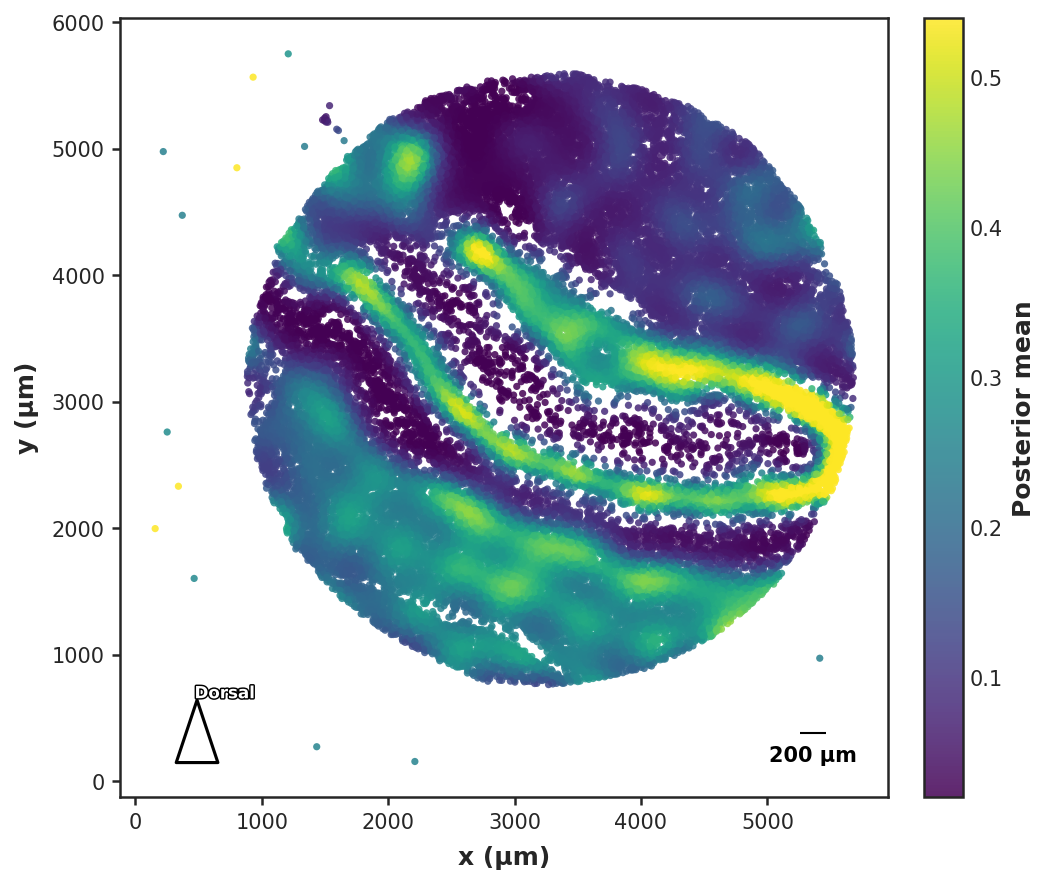
\includegraphics[height=0.7\textheight,keepaspectratio]
        {SLC17A7_Classifier.png}
        
      \vspace{1ex}
      % tiny caption
      {\tiny\textbf{(a)} EFGP Classification Fit - approx. $45$s for 50 GD iters}
      \end{columns}

\end{frame}

\begin{frame}{Summary}
    Built on Equispaced Fourier Features from Greengard et al.\\
    Results: 
    \begin{enumerate} 
    \item $\mathcal O(n + m\log m)$ algorithms for learning kernel hyperparameters and fitting Gaussian, Bernouli, or Negative Binomial observations using Equispaced Fourier Features 
    \item More than $10x$ faster than best fast-GP predecessors for low-dimensional problems in conjugate case on a spatial transcriptomics task
    \item Efficient variance calculations
    \item Usable software!
    \end{enumerate}
\end{frame}

\begin{frame}{Next Steps}
    \begin{enumerate}
        \item Scaling performance of EFGP on GPUs
        \item Application of EFGP to other GP methods-- eg EFGP + inducing points.
        \item Applied problem with $n$ large, $d\leq 3$?
    \end{enumerate}
\end{frame}
\begin{frame}{Thank yous}
  \begin{columns}[c] % vertically center the content of each column
    \column{0.33\textwidth}
      \centering
      \includegraphics[width=0.6\linewidth]{scott_small.jpg}
      \captionof{figure}{Scott Linderman\\ (Stanford)}

    \column{0.33\textwidth}
      \centering
      \includegraphics[width=0.6\linewidth]{Dan.jpg}
      \captionof{figure}{Dan Biderman\\(Stanford)}
    \column{0.33\textwidth}
      \centering
      \includegraphics[width=0.7\linewidth]{pgreengard.png}
      \captionof{figure}{Philip Greengard\\(Flatiron Institute)}

  \end{columns}
\end{frame}
\section{Additional Slides}
\begin{frame}{Misc}
\end{frame}
\begin{frame}{Computational Bottleneck}
    Throughout E and M steps, need to solve the following for $v$:

    $$(K^{-1} + \Delta )v = z$$
Strategy:
\begin{enumerate}
    \item Can rewrite as $m$-dimensional system by solving for $u$ by CG, then recover $v = \Phi u$.

    $$(I + \Phi^* \Delta \Phi) u =\Phi^* z $$
    \item  We can speed up this solve by preconditioning with the approximation $\Delta = \bar \delta I$ where $\bar \delta$ is the mean of the $\Delta$ diagonal matrix. This cuts down computations dramatically if $\Delta$ is anywhere close to constant. Ie solve
  $$(I + \bar{\delta} \Phi^* \Phi)u = \Phi^* z$$
  In some arbitrary case I tested, from 100 $\mathcal O(n)$ CG iters down to 7. 
    \end{enumerate}
\end{frame}
\begin{frame}{Bibliography}
    \bibliography{refs}           % <-- no “.bib”

\end{frame}



\end{document}